\section{Results}
\subsection{Automatic generation of PH model from the PID network}
%give statistics
PH models are written using the PINT\footnote{\url{http://process.hitting.free.fr}} format.  
PINT implements stochastic simulations and static analyses for computing dynamical properties on very large-scale PH models.
For the PINT code generation two procedures were used.
The first procedure detects motifs (controller and controlled components) in graphs from the Pathway Interaction Database; the second, 
generates the PINT code by choosing an adequate concurrency rule, based on synchronization sorts, to represent the motif dynamic in PH.
With this method it is possible to convert the whole content of the PID database into a PH model, as well as individual pre-selected pathways, 
as is the case for the system under study.  It is implemented in Java and available upon request.
%taking in consideration the type of the pattern to better refine the dynamic of the system from a structural point of view.
%This refinement is done by introducing the synchronization sort  which is a generalization of the cooperation sort. This allows  to avoid artificial oscillations
%in the dynamics of the components of the system.

\subsection{Simulation of Calcium stimulated biological system}
We simulated the model with and without the inclusion of the synchronization sort. In the following, we present the results of 
the simulation.

\subsubsection{Without the introduction of the synchronization sort.}
One can notice in \pref{fig:rwos} the occurrence of oscillations. Whereas it is not the expected behavior from the biological system,
 it is coherent with the choice of the modeling and the way the simulator works as explained in Section \ref{sssec:synchronization}.
In this simulation, cooperation sorts were used to model multiple controllers of a common controlled (target) component.
%In other cases we left the components act independently.
It is important to notice that the intensity of the oscillation is linked with 
the size of the concurrence, i.e. the number of controllers a controlled component has.
Despite the presence of the oscillations, the model reproduces expected dynamical behaviors  namely
the dynamics of components, the signal transduction and takes into account the stochastic and time aspect of the model.

\begin{figure}[H]
\centering
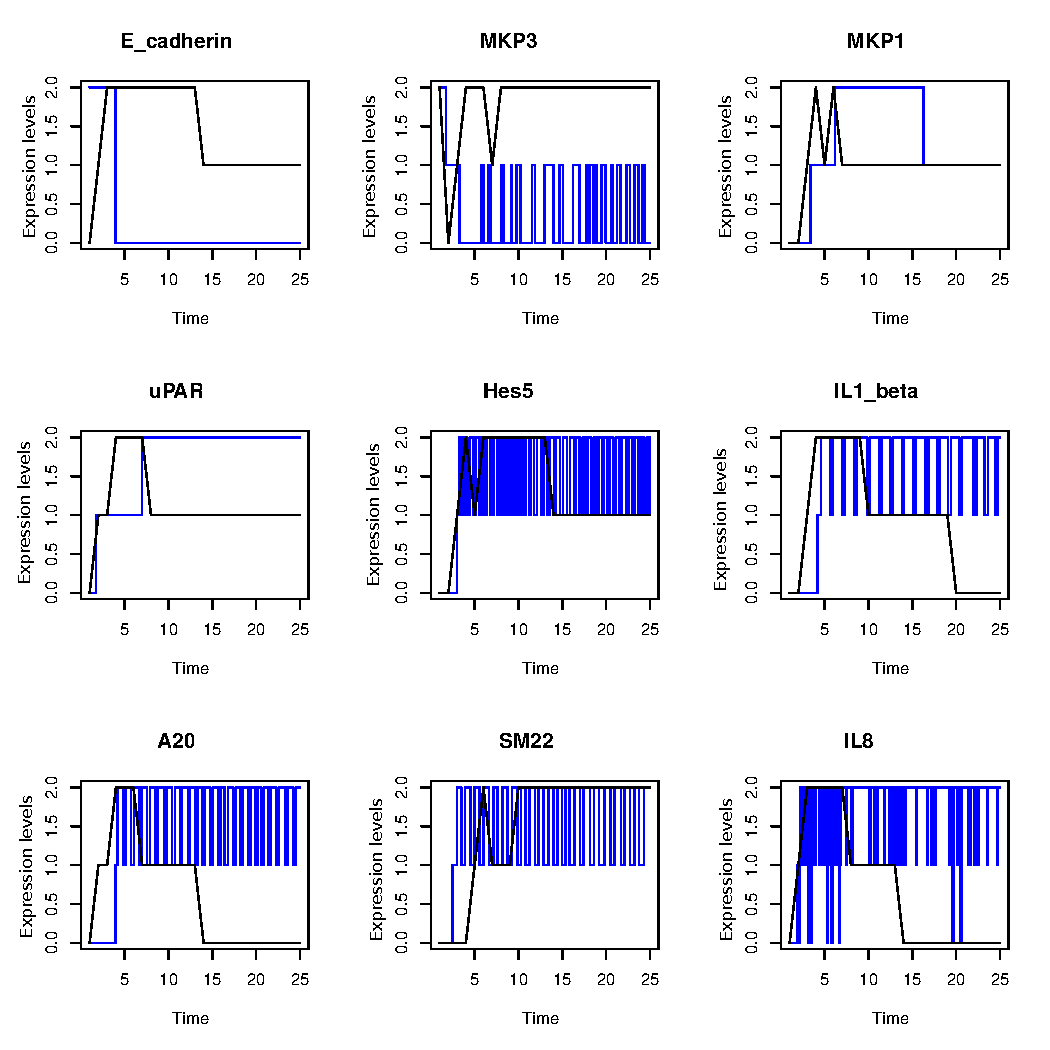
\includegraphics[width=5in,height=4in]{images/resultWOS.pdf}
\caption{{\bf Results of system simulations without introducing the synchronization sort for 9 genes.} The 
traces representing the discretized time-series data are shown as black lines.  The traces representing the simulated traces are shown as blue lines.}
\label{fig:rwos}
\end{figure}

\subsubsection{With the introduction of the synchronization sort.}
In \pref{fig:rws} we can see that the introduction of the synchronization sort significantly reduces the 
impact of concurrency. The result shows  a 
clear elimination of the previously observed oscillations (\pref{fig:rwos}). 
Comparing the simulated results with the ones observed experimentally, we found four different cases.
We found $5$ simulation traces (IL8, uPAR, IL1\_beta, ET1, A20) that matched the sequence of all the component expression levels perfectly.  In this case, delays exist among simulation and experiment but 
these delays are not comparable since experimental time-points are measured in hours and simulation-units for the simulated PH model.
We found $6$ simulation traces (MKP1, MKP3, Hes5, SM22, TfR, DKK1) that matched the sequence of experimental discrete expression levels missing one expression-level.
We found $1$ components (TNF-alpha) in which at least 2 expression levels are missed.
%Finally we found 1 component (A20) for which we did not reproduce its experimentally observed dynamics.


%The expression levels of genes \emph{uPAR}, \emph{MKP1},
%\emph{IL1-beta} are well reproduced, while \emph{Hes5} and \emph{IL8} are not activated. This result can be observed when the activation
%signal has not been able to propagate through the network due to the non determinism  and concurrency.


\begin{figure}[H]
\centering
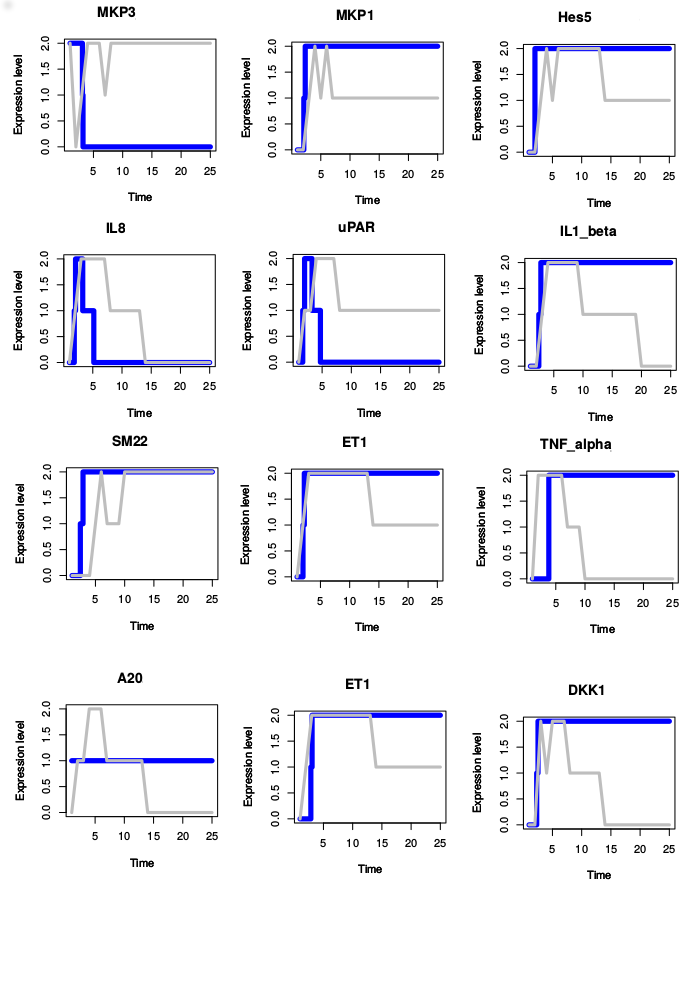
\includegraphics[width=5in,height=7in]{images/12genes_sim.png}
\caption{{\bf Results of simulations by introducing the synchronization sort.} The gray traces represent the experimental expected behaviors
from the discretization of the time-series data. The blue traces show the simulated behavior.}
\label{fig:rws}
\end{figure}


%%%%%images des noeuds clés

\subsubsection{Simulating biological processes.}
To validate our model, we studied the prediction of non-observed components of such a system and we focused on biological processes linked 
to Calcium stimulation, such as keratinocyte-differentiation, cell-adhesion and cell-cycle arrest.
Our results are shown in \pref{fig:knodes} and confirm literature experimental evidences on these processes.
In the case of keratinocyte-differentiation, this was a functional behavior measured on the cultured cells upon Calcium stimulation,
 so there was experimental evidences of this effect before measuring the gene expression.  
In the case of cell-cycle arrest, the switch-on of this component represents the fact that the E-cadherin stimulated model predicts the stop 
of growth, as confirmed by literature in human and mouse keratinocytes~\cite{Kolly2005}.
Finally, the cell-adhesion component is predicted to switch-on, also in according to published evidence~\cite{Tu2011} in human and mouse keratinocytes.

\begin{figure}[H]
\centering
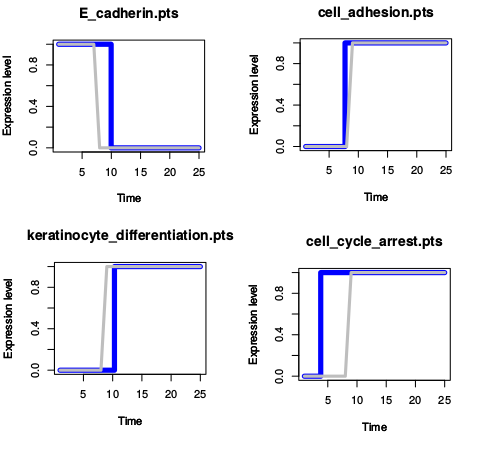
\includegraphics[width=4in,height=3.5in]{images/key_nodes1.png}
\caption{{\bf Results of the prediction of biological processes.} The gray traces represent the experimental and literature-based evidence.
The blue traces show the simulated behavior of E-cadherin and three biological processes.}
\label{fig:knodes}
\end{figure}

%to answer the question of confidence in the result of simulation
\subsection{Model validation: traces analysis}
\modCG{
To validate the results of the simulations, we automatically analyzed the traces generated by a set of $100$ simulations. Table \ref{traceAnalysis} shows the results
of the percentage of acceptance for the traces of each of the $12$ mRNA expression. One can observed that, there are components with a good 
rate of acceptance (A20, IL1$\_$beta, IL8, uPar). The reason is probably that they have traces that are more simple to reproduce. Another observation is that they 
are others components which have low rate of acceptance (ET1, DKK1, MKP1, MKP3). We think that their traces are more complicate to reproduce.
But in all the case the rate of acceptance increase with tolerance in  automatic verification.  
}

\begin{table}[!t]
\renewcommand{\arraystretch}{1.3}

\caption{Percentage of acceptance traces. First column represents the Automaton ($\mathcal{A}_{i}(w)$, where $\mathcal{A}_{i}$ is the Automaton and $w$ is the word recognized by $\mathcal{A}_{i}$) 
that is used to check if a given trace is acceptance for a component in the second 
column. One can observed that many components can be recognized by the same Automaton. In the third column we have the percentage of acceptance traces. Finally in the fourth column
are the percentage of acceptance with a tolerance of one level ($T_{1}$)}

\label{traceAnalysis}
\centering
%table of result
\begin{tabular}{|c|c||c|c|}
\hline

\textbf{Automate}

&

\textbf{components}

&

\textbf{$\%$ of acceptance}

&

\textbf{$\%$ of acceptance $T_{1}$}
\\ \hline

$\mathcal{A}_{2}(01210)$

&

A20

&

91

&

100
\\ \hline

$\mathcal{A}_{2}(01210)$

&

IL1$\_$beta

&

81

&

100
\\ \hline

$\mathcal{A}_{2}(01210)$

&

IL8

&

93

&

100

\\ \hline

$\mathcal{A}_{2}(01210)$

&

TNF$\_$alpha

&

0

&

0

\\ \hline

$\mathcal{A}_{3}(01211)$

&

uPar

&

76

&

99

\\ \hline

$\mathcal{A}_{3}(01211)$

&

ET1

&

8

&

19

\\ \hline

$\mathcal{A}_{4}(0121210)$

&

DKK1

&

13

&

43

\\ \hline

$\mathcal{A}_{5}(0121211)$

&

Hes5


&

0

&

17

\\ \hline

$\mathcal{A}_{5}(0121211)$

&

MKP1


&

9

&

97

\\ \hline

$\mathcal{A}_{6}(0212)$

&

SM22


&

11

&

100

\\ \hline

$\mathcal{A}_{7}(02010)$

&

MKP3


&

11

&

98

\\ \hline

$\mathcal{A}_{8}(02121)$

&

Tfr


&

0

&

94

\\ \hline

 
\end{tabular}
\end{table}








% An example of a floating figure using the graphicx package.
% Note that \label must occur AFTER (or within) \caption.
% For figures, \caption should occur after the \includegraphics.
% Note that IEEEtran v1.7 and later has special internal code that
% is designed to preserve the operation of \label within \caption
% even when the captionsoff option is in effect. However, because
% of issues like this, it may be the safest practice to put all your
% \label just after \caption rather than within \caption{}.
%
% Reminder: the "draftcls" or "draftclsnofoot", not "draft", class
% option should be used if it is desired that the figures are to be
% displayed while in draft mode.
%
%\begin{figure}[!t]
%\centering
%\includegraphics[width=2.5in]{myfigure}
% where an .eps filename suffix will be assumed under latex, 
% and a .pdf suffix will be assumed for pdflatex; or what has been declared
% via \DeclareGraphicsExtensions.
%\caption{Simulation Results}
%\label{fig_sim}
%\end{figure}

% Note that IEEE typically puts floats only at the top, even when this
% results in a large percentage of a column being occupied by floats.


% An example of a double column floating figure using two subfigures.
% (The subfig.sty package must be loaded for this to work.)
% The subfigure \label commands are set within each subfloat command, the
% \label for the overall figure must come after \caption.
% \hfil must be used as a separator to get equal spacing.
% The subfigure.sty package works much the same way, except \subfigure is
% used instead of \subfloat.
%
%\begin{figure*}[!t]
%\centerline{\subfloat[Case I]\includegraphics[width=2.5in]{subfigcase1}%
%\label{fig_first_case}}
%\hfil
%\subfloat[Case II]{\includegraphics[width=2.5in]{subfigcase2}%
%\label{fig_second_case}}}
%\caption{Simulation results}
%\label{fig_sim}
%\end{figure*}
%
% Note that often IEEE papers with subfigures do not employ subfigure
% captions (using the optional argument to \subfloat), but instead will
% reference/describe all of them (a), (b), etc., within the main caption.


% An example of a floating table. Note that, for IEEE style tables, the 
% \caption command should come BEFORE the table. Table text will default to
% \footnotesize as IEEE normally uses this smaller font for tables.
% The \label must come after \caption as always.
%
%\begin{table}[!t]
%% increase table row spacing, adjust to taste
%\renewcommand{\arraystretch}{1.3}
% if using array.sty, it might be a good idea to tweak the value of
% \extrarowheight as needed to properly center the text within the cells
%\caption{An Example of a Table}
%\label{table_example}
%\centering
%% Some packages, such as MDW tools, offer better commands for making tables
%% than the plain LaTeX2e tabular which is used here.
%\begin{tabular}{|c||c|}
%\hline
%One & Two\\
%\hline
%Three & Four\\
%\hline
%\end{tabular}
%\end{table}


% Note that IEEE does not put floats in the very first column - or typically
% anywhere on the first page for that matter. Also, in-text middle ("here")
% positioning is not used. Most IEEE journals/conferences use top floats
% exclusively. Note that, LaTeX2e, unlike IEEE journals/conferences, places
% footnotes above bottom floats. This can be corrected via the \fnbelowfloat
% command of the stfloats package.
